\documentclass[11pt,twocolumn]{article}

\usepackage{array}
\usepackage[url=false, doi=false]{biblatex}
\usepackage{booktabs}
\usepackage[font=footnotesize, labelfont=bf]{caption}
\usepackage{enumitem}
\usepackage[symbol]{footmisc}
\usepackage[scale=0.85]{geometry}
\usepackage{lipsum}
\usepackage{microtype}
\usepackage{multirow}
\usepackage{parskip}
\usepackage{siunitx}
\usepackage{titlesec}
\usepackage[dvipsnames]{xcolor}
\usepackage{xurl}
\usepackage[hidelinks]{hyperref}
\usepackage[nameinlink,capitalise]{cleveref}
\usepackage{verbatim}
\usepackage{graphicx}
\usepackage{float}

\addbibresource{../bibliography.bib}

\titlelabel{}

\newcommand{\atom}[1]{\colorbox{Gray!30}{\ttfamily #1}}
\newcommand{\citen}[1]{~\parencite{#1}}
\newcommand{\citeay}[1]{\textcite{#1}}
\newcommand{\winner}[1]{{\bfseries\color{ForestGreen}#1}}

\pagenumbering{gobble}

\setlist[enumerate]{itemsep=1pt, topsep=1pt, parsep=0pt, partopsep=0pt}

\setcounter{footnote}{1}

\title{Tableaux Resetmaxxing}
\date{}
\author{}

\begin{document}
\twocolumn[
	\centering
	\vspace{1em}
	{\LARGE\bfseries Tableau Resetmaxxing for Fun and Profit \par} \vspace{3pt}
	{\large (a crazy idea that works really well) \par}
	\vspace{2em}
]
% \maketitle

\section{Introduction and Novel Idea}

\citeauthor{eliminatingModels} introduce SATCoP\citen{eliminatingModels}, a tableau prover based on LeanCoP\citen{Otten2023leanCoP20} that runs a separate SAT solver along fed with grounded atoms from the tableau prover.
If the SAT solver reaches an unsatisfiable state, then we can prove that the entire tree is unsatisfiable.

However, other than the underlying SAT solver, the tableau prover in the implementation of SATCoP only has a few improvements over the original LeanCoP.
\begin{enumerate}
	\item Randomisation of literals at \atom{Start} and \atom{Extension} clauses.
	\item Deepening control: only increase maximum height when the SAT model is stale.
	\item And a big improvements present in \textbf{9.1 A Note from the Future} and in CASC: SAT-guided preference: reorder extensions by the SAT model's opinions of the literals.
	\label{satsolvelit_description}
\end{enumerate}

I improved the current model of \atom{SATSolve} with the reordering in \cref{satsolvelit_description} to generate \atom{SATSolveLiteral}.
This already provides a big improvement over the baseline.

For the most part, this guidance tries to maximise the chance of closing the tableau rather than trying to create UNSAT on the underlying SAT solver.

While experimenting with choices for SAT-based guidance\cite{apr22_pres}, I found some big improvements in specifically changing the tableau search to achieve this.
In particular, \textbf{resetting the tableau search early and often to generate different statements for the SAT solver considerably improves the overall model}.

This makes some sense intuitively: instead of trying to close the tableau, we are trying to generate the maximum amount of valid SAT statements to ``close'' the SAT prover.

As far as I can tell this is sound (althrough very incomplete).

\section{Implementation}

We compare these strategies for the SAT prover along with two control strategies: \atom{FirstAction} and \atom{LeanCoPCut}.

	\begin{enumerate}
		\item \atom{SATSolve}  Plain SATCoP\cite{eliminatingModels}. Last week's best model.
		\item \atom{SATSolveLiteral}  SATCoP with the extension reordering.
		\item \atom{SATResetAtStaleAction} Reset when no new actions to the SAT solver.
		\item \atom{SATResetAtStaleBacktrack} Reset when backtracking if no new actions have been added to the SAT solver.
		\item \atom{SATResetBandit}  Tiny contextual bandit choosing between \atom{Backtrack(1)}, \atom{Backtrack(2)}, and \atom{Reset(n + 1)} depending on whether the shadow CNF is still growing.
	\end{enumerate}

\section{Overall Results}

The CRS3 tier is currently hammered, so most of these tests were done locally with a small 60 second time limit and 1 million step limit.

\begin{figure}[h]
	\centering
	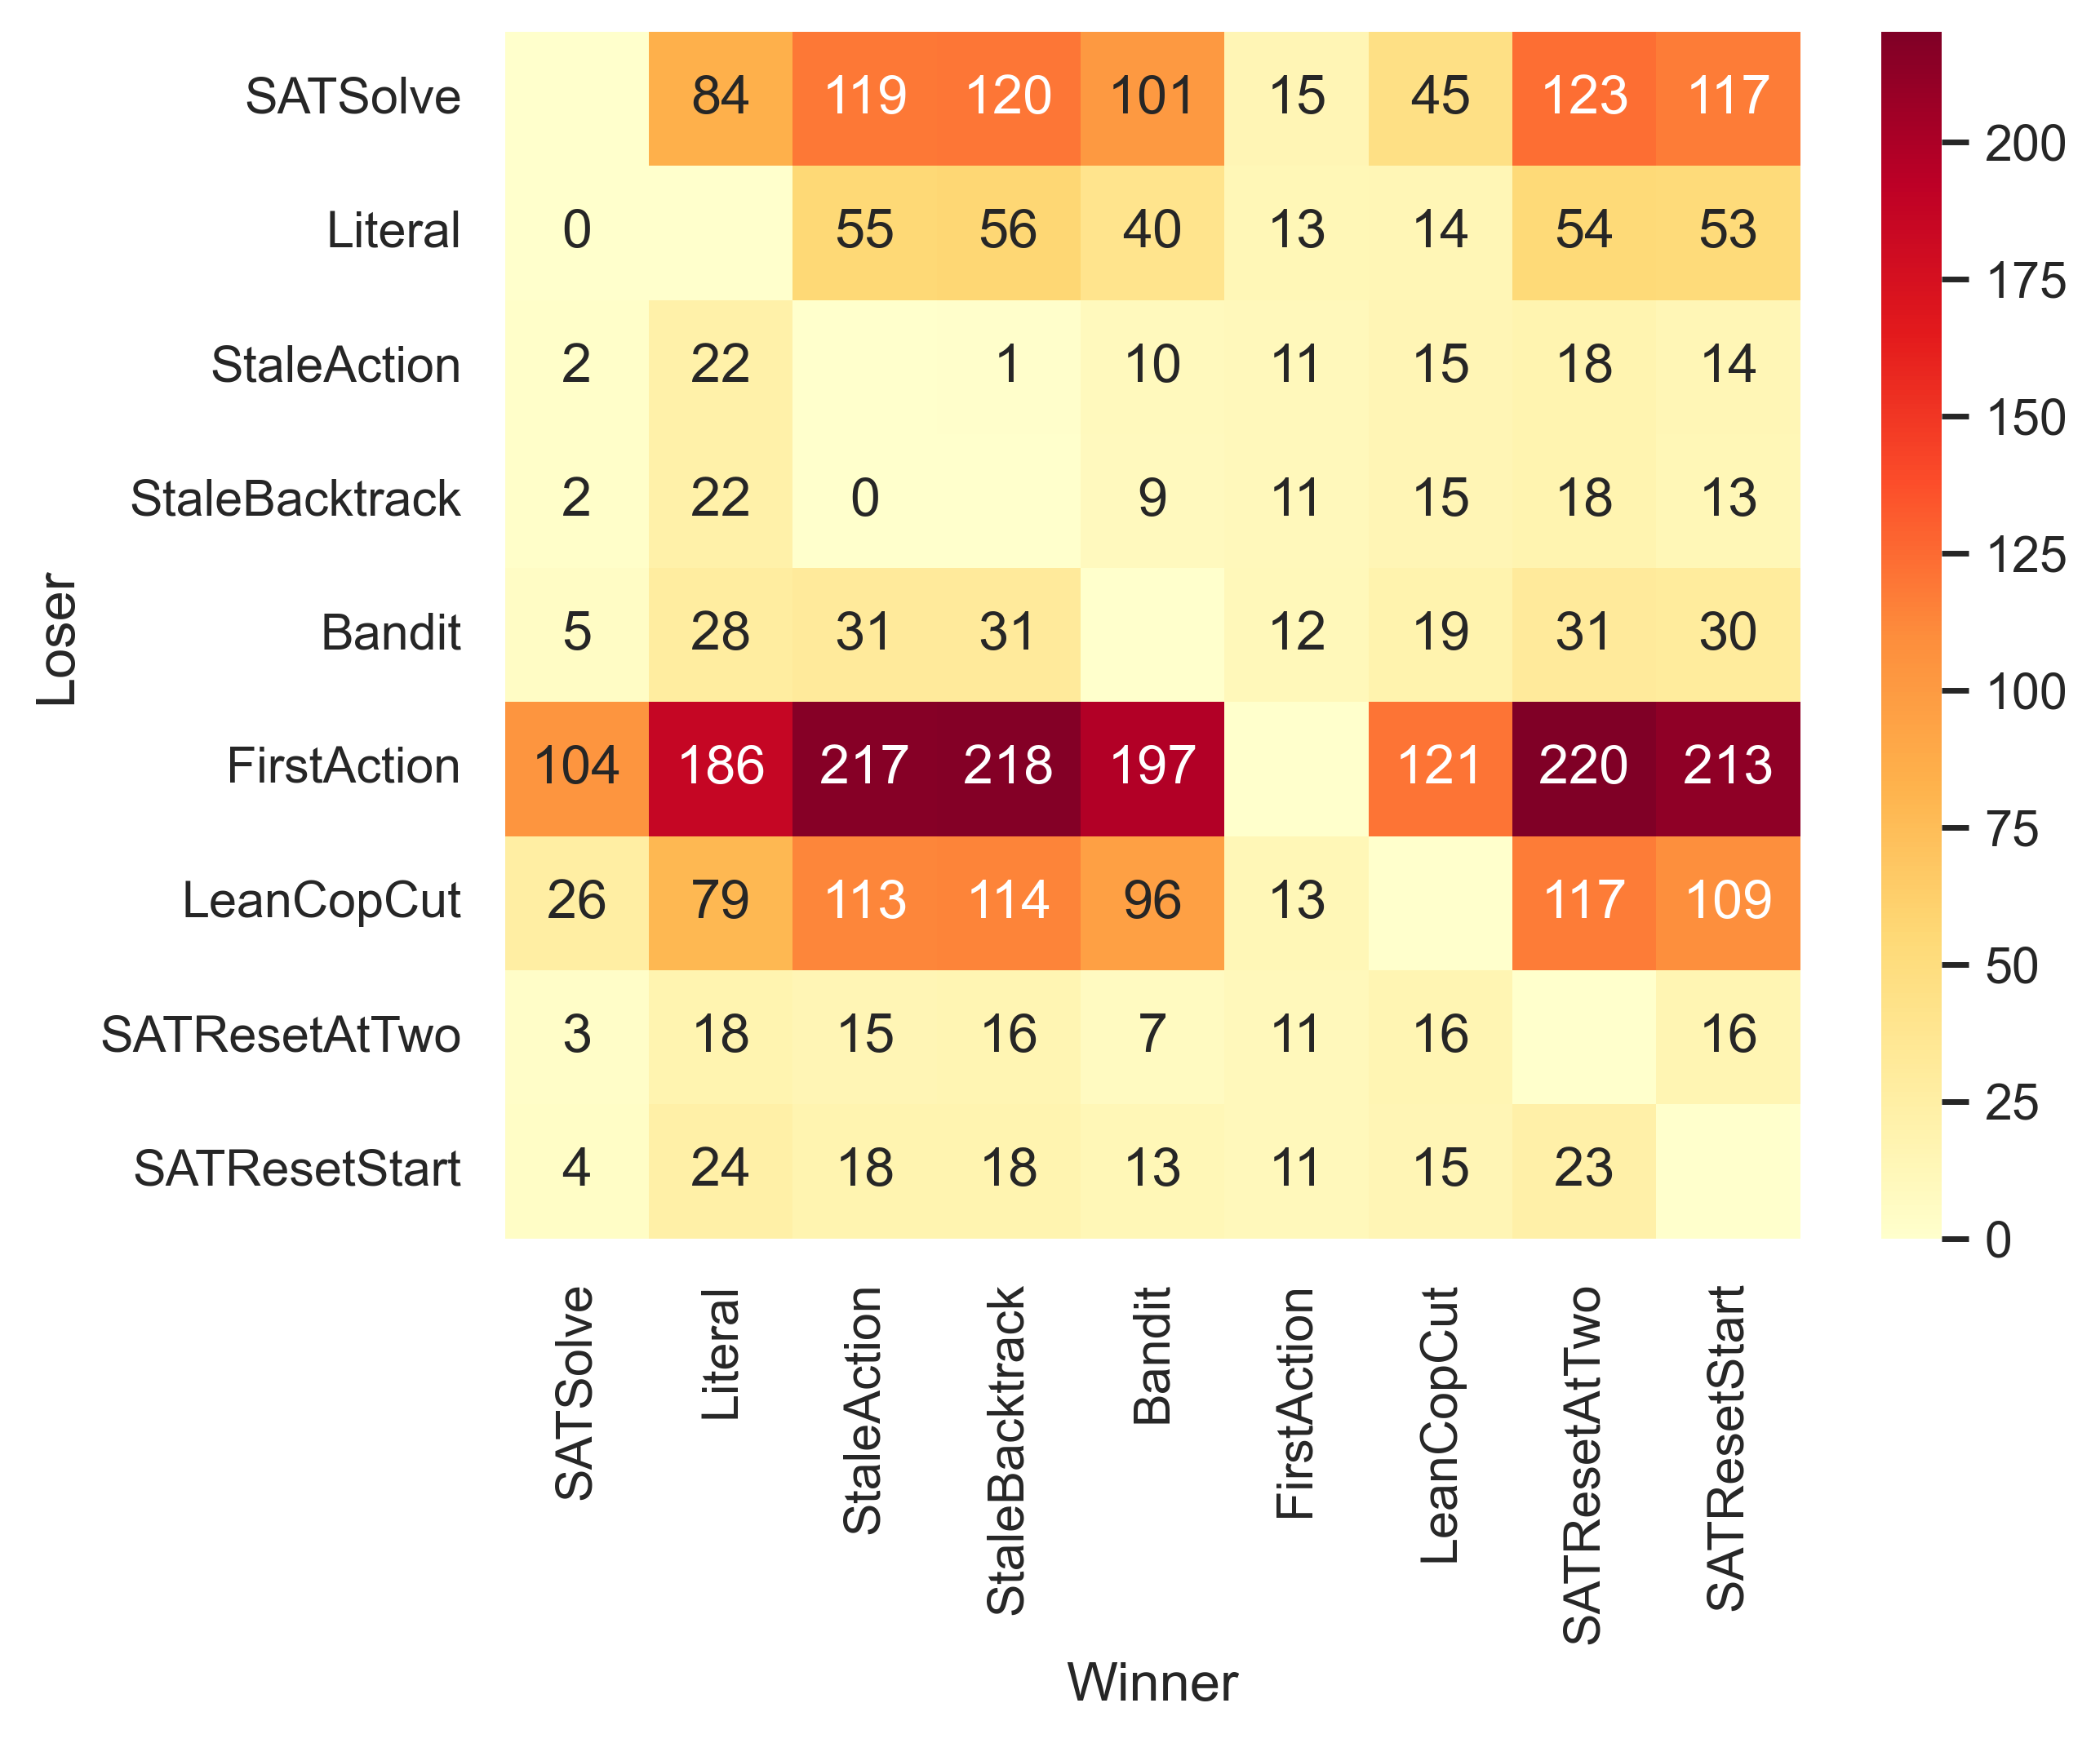
\includegraphics[width=\columnwidth]{../../figures/sat_policies_plot_29Apr.png}
	\caption{Winners and losers of the strategies in a representative subset of 501 problems by \citeay{chvalovsky2021characteristic}.}
\end{figure}

\section{Some Interesting Results}

% \newcommand{\MS}{{\color{BrickRed}\bfseries max-steps}}
% \newcommand{\TO}{{\color{OrangeRed}\bfseries timeout}}
% \newcommand{\best}{\color{Green}}
% 
% \sisetup{
%     table-format = 11.0,
% 	table-text-alignment = right,
% }
% 
% \setlength{\defaultaddspace}{4pt}

\begin{table*}[t]
	\centering
	\scriptsize
	\begin{tabular}{>{\ttfamily\bfseries}l *{7}{rr}}
		\toprule
		\multirow{2}{*}{{\rmfamily\bfseries Problem}}
			& \multicolumn{2}{c}{\atom{FirstAction}}
			& \multicolumn{2}{c}{\atom{LeanCoPCut}}
			& \multicolumn{2}{c}{\atom{SATSolve}}
			& \multicolumn{2}{c}{\atom{Literal}}
			& \multicolumn{2}{c}{\atom{StaleAction}}
			& \multicolumn{2}{c}{\atom{StaleBacktrack}}
			& \multicolumn{2}{c}{\atom{Bandit}} \\
		& {\bfseries time} & {\bfseries steps}
		& {\bfseries time} & {\bfseries steps}
		& {\bfseries time} & {\bfseries steps}
		& {\bfseries time} & {\bfseries steps}
		& {\bfseries time} & {\bfseries steps}
		& {\bfseries time} & {\bfseries steps}
		& {\bfseries time} & {\bfseries steps} \\
		\midrule
			CSR052+1.p & \multicolumn{2}{c}{---} & \multicolumn{2}{c}{---} & \multicolumn{2}{c}{---} & 31s & 35,616 & 1s & 149 & \winner{1s} & \winner{149} & 1s & 277 \\
			GEO185+3.p & \multicolumn{2}{c}{---} & \multicolumn{2}{c}{---} & \multicolumn{2}{c}{---} & \multicolumn{2}{c}{---} & \winner{11s} & \winner{3,899} & 13s & 3,900 & 17s & 3,583 \\
			GEO202+3.p & \multicolumn{2}{c}{---} & 26s & 13,927 & \multicolumn{2}{c}{---} & \multicolumn{2}{c}{---} & \winner{7s} & \winner{2,222} & 7s & 2,222 & 10s & 2,399 \\
			GEO233+1.p & \multicolumn{2}{c}{---} & \multicolumn{2}{c}{---} & \multicolumn{2}{c}{---} & \multicolumn{2}{c}{---} & 14s & 3,219 & 14s & 3,219 & \winner{7s} & \winner{1,870} \\
			GEO262+3.p & \multicolumn{2}{c}{---} & \multicolumn{2}{c}{---} & \multicolumn{2}{c}{---} & \multicolumn{2}{c}{---} & 7s & 1,802 & \winner{6s} & \winner{1,802} & 8s & 2,696 \\
			\addlinespace
			HWV025-2.p & \multicolumn{2}{c}{---} & \multicolumn{2}{c}{---} & 50s & 7,392 & 35s & 8,025 & 8s & 1,151 & \winner{7s} & \winner{1,151} & \multicolumn{2}{c}{---} \\
			\addlinespace
			KRS072+1.p & \multicolumn{2}{c}{---} & \multicolumn{2}{c}{---} & \multicolumn{2}{c}{---} & \multicolumn{2}{c}{---} & \winner{3s} & \winner{1,605} & 4s & 1,605 & 9s & 3,028 \\
			KRS162+1.p & \multicolumn{2}{c}{---} & \multicolumn{2}{c}{---} & \multicolumn{2}{c}{---} & \multicolumn{2}{c}{---} & 21s & 4,486 & 22s & 4,486 & \winner{19s} & \winner{4,431} \\
			KRS167+1.p & 59s & 30,732 & \multicolumn{2}{c}{---} & 15s & 5,307 & 16s & 15,277 & 5s & 2,042 & 5s & 2,042 & \winner{2s} & \winner{658} \\
			\addlinespace
			LCL126-1.p & \multicolumn{2}{c}{---} & \multicolumn{2}{c}{---} & \multicolumn{2}{c}{---} & 24s & 2,415 & \winner{3s} & \winner{742} & 3s & 742 & \multicolumn{2}{c}{---} \\
			\addlinespace
			NUM337+1.p & \multicolumn{2}{c}{---} & \multicolumn{2}{c}{---} & \multicolumn{2}{c}{---} & \multicolumn{2}{c}{---} & 40s & 5,185 & \winner{37s} & \winner{5,185} & \multicolumn{2}{c}{---} \\
			NUM411+1.p & \multicolumn{2}{c}{---} & 45s & 26,538 & \multicolumn{2}{c}{---} & \multicolumn{2}{c}{---} & 6s & 2,850 & 6s & 2,850 & \winner{1s} & \winner{659} \\
			NUM432+3.p & 11s & 5,052 & 8s & 4,010 & \multicolumn{2}{c}{---} & 60s & 21,655 & 2s & 914 & 2s & 914 & \winner{2s} & \winner{462} \\
			\addlinespace
			RNG089+2.p & 24s & 5,771 & 23s & 5,441 & 27s & 4,476 & 11s & 4,907 & \winner{1s} & \winner{339} & 2s & 339 & 35s & 4,025 \\
			\addlinespace
			SET027-7.p & \multicolumn{2}{c}{---} & \multicolumn{2}{c}{---} & \multicolumn{2}{c}{---} & \multicolumn{2}{c}{---} & 49s & 6,346 & \winner{42s} & \winner{6,346} & 55s & 7,685 \\
			SET114-7.p & 5s & 1,632 & 5s & 1,632 & 22s & 4,698 & 11s & 4,690 & 1s & 123 & \winner{1s} & \winner{123} & 33s & 3,739 \\
			SET602+4.p & \multicolumn{2}{c}{---} & \multicolumn{2}{c}{---} & \multicolumn{2}{c}{---} & \multicolumn{2}{c}{---} & \multicolumn{2}{c}{---} & \multicolumn{2}{c}{---} & \winner{27s} & \winner{3,503} \\
			SET677+3.p & \multicolumn{2}{c}{---} & \multicolumn{2}{c}{---} & \multicolumn{2}{c}{---} & 33s & 11,136 & 1s & 340 & \winner{1s} & \winner{340} & 2s & 366 \\
			\addlinespace
			SEU121+2.p & \multicolumn{2}{c}{---} & 43s & 29,479 & \multicolumn{2}{c}{---} & 46s & 42,182 & 11s & 3,396 & \winner{7s} & \winner{3,396} & 19s & 4,714 \\
			SEU234+1.p & \multicolumn{2}{c}{---} & \multicolumn{2}{c}{---} & 31s & 10,262 & 32s & 30,860 & 14s & 6,563 & 14s & 6,563 & \winner{11s} & \winner{4,236} \\
			\addlinespace
			SWC136+1.p & \multicolumn{2}{c}{---} & \multicolumn{2}{c}{---} & \multicolumn{2}{c}{---} & \multicolumn{2}{c}{---} & \winner{13s} & \winner{2,982} & 19s & 2,982 & 16s & 2,078 \\
			\addlinespace
			SWV908-1.p & \multicolumn{2}{c}{---} & \multicolumn{2}{c}{---} & \multicolumn{2}{c}{---} & \multicolumn{2}{c}{---} & \winner{14s} & \winner{1,286} & 17s & 1,286 & 22s & 1,315 \\
			\addlinespace
			SYN154-1.p & \multicolumn{2}{c}{---} & \multicolumn{2}{c}{---} & 38s & 9,279 & 37s & 18,150 & 1s & 95 & \winner{1s} & \winner{95} & 2s & 550 \\
			SYN158-1.p & \multicolumn{2}{c}{---} & \multicolumn{2}{c}{---} & \multicolumn{2}{c}{---} & 33s & 17,984 & 4s & 1,394 & 4s & 1,394 & \winner{3s} & \winner{1,106} \\
			SYN163-1.p & \multicolumn{2}{c}{---} & \multicolumn{2}{c}{---} & \multicolumn{2}{c}{---} & \multicolumn{2}{c}{---} & \winner{6s} & \winner{2,074} & 6s & 2,074 & 11s & 2,827 \\
			SYN209-1.p & \multicolumn{2}{c}{---} & \multicolumn{2}{c}{---} & \multicolumn{2}{c}{---} & 55s & 26,905 & \winner{1s} & \winner{481} & 1s & 481 & 4s & 1,260 \\
			SYN260-1.p & 7s & 4,126 & 6s & 4,126 & 32s & 8,794 & 16s & 9,156 & \winner{2s} & \winner{845} & 3s & 845 & 10s & 2,874 \\
			SYN625-1.p & \multicolumn{2}{c}{---} & \multicolumn{2}{c}{---} & \multicolumn{2}{c}{---} & 42s & 18,502 & 14s & 2,312 & \winner{12s} & \winner{2,312} & \multicolumn{2}{c}{---} \\
			SYN669-1.p & \multicolumn{2}{c}{---} & \multicolumn{2}{c}{---} & \multicolumn{2}{c}{---} & \multicolumn{2}{c}{---} & 3s & 1,082 & 3s & 1,082 & \winner{2s} & \winner{582} \\
			SYN677-1.p & \multicolumn{2}{c}{---} & \multicolumn{2}{c}{---} & \multicolumn{2}{c}{---} & \multicolumn{2}{c}{---} & 9s & 2,841 & 8s & 2,842 & \winner{2s} & \winner{708} \\
		\bottomrule
	\end{tabular}
	\caption{Thirty interesting problems for comparing these programs. All tested locally; step count should be accurate, time likely is not.}
	\label{tab:reset-wins}
\end{table*}

% A subset of 247 ``representative'' TPTP problems was used for evaluation\citen{chvalovsky2021characteristic}.
% The results with any significance are found in \cref{big_table}.
% 
% The comparer runs all 6 policies in parallel, with a 30-second time limit and a \num{50000} step limit.
% A larger experiment, with the entirety of TPTP and a longer time limit, will come in the future.
% 
% I also post-process the canonical TPTP runs into short serial schedules.
% For each strategy and time cap, the pair ``strategy + cap'' is treated as covering exactly the problems that the strategy solves within that cap.
% The schedule synthesis problem is therefore a budgeted maximum-coverage problem with a multiple-choice knapsack constraint: choose at most one cap per strategy, subject to a global budget of 60 or 120 seconds, and maximise either the total number of solved problems or the number of solved problems outside LeanCopCut's solved set.
% After fixing the capped strategies, I then order them by a second optimisation pass that minimises total runtime over the benchmark set, using the recorded per-problem runtimes and charging the full cap on timeout rows.
% 
% The results show that all three policies have marked improvements in certain problems.
% It's likely that with further exploration we might get even better results than the control groups.

\renewcommand*{\bibfont}{\small}
\printbibliography{}

\end{document}
